\documentclass[11pt]{article}
\usepackage[margin=2.2cm]{geometry}
\usepackage{amsmath,amssymb,booktabs,enumitem,graphicx}
\usepackage[hidelinks]{hyperref}
\setlist{nosep,leftmargin=*}
\setlength{\parindent}{0pt}
\graphicspath{{results/default/regime_analysis/}}

\newcommand{\dt}{\tilde\delta}
\newcommand{\nb}{\bar n}

\title{From analysis to model: a cascade for point-process inference}
\date{}

\begin{document}
\maketitle

%==============================================================================
\section{The pitch}

\begin{itemize}
  \item AISTATS is an ML venue: a \textbf{new model} that solves a problem is a stronger paper than an analysis of where existing models fail
  \item This does not discard the previous work, it \textbf{uses} it: the regime analysis in \texttt{results/} identified the failure mode, and the new model is designed around it
  \item One-line summary: \emph{first decide whether there is any structure to infer, and only then infer it, with every downstream model trained on data where the structure is actually visible}
\end{itemize}

%==============================================================================
\section{What the exploration showed}

The previous runs (\texttt{docs/05\_results}) compared 22 feature sets (classical summary functions, persistent homology) on 5-way classification and parameter estimation. The consistent finding:

\begin{itemize}
  \item \textbf{Everything breaks in the same place: near complete spatial randomness (CSR).}
  \begin{itemize}
    \item Below $\dt\approx0.6$ every method fails on Thomas (recall $0.03$--$0.19$, below chance), calling $56$--$71\%$ of those patterns Poisson
    \item The lowest-$\dt$ bins are below chance for every feature set; the modal prediction there is Poisson
    \item Parameter errors are largest near CSR and shrink as the structure strengthens (Thomas log-RMSE $1.22 \to 0.46$, LGCP $0.89 \to 0.30$ across the $\dt$ range)
  \end{itemize}
  \item \textbf{No feature set fixes it.} Classical and topological inputs fail together, so the limit is information in the pattern, not the model
  \item \textbf{Conclusion:} don't fight the near-CSR regime --- route around it
\end{itemize}

%==============================================================================
\section{Design philosophy}

\begin{center}
\begin{tabular}{@{}lll@{}}
\toprule
stage & question & trained on \\
\midrule
1. filter      & Poisson, clustered or repulsive?          & all simulated clouds \\
2. classifier  & which clustered family? (Thomas, nested, LGCP) & clustered clouds \emph{past the cutoff} \\
3. estimators  & the family's parameters (one model per family) & that family's clouds \emph{past the cutoff} \\
\bottomrule
\end{tabular}
\end{center}

\begin{itemize}
  \item A Poisson call needs no model: the intensity estimate $\hat{\nb} = n$ is the exact MLE. The repulsive group has one family (Mat\'ern II), so it needs no classifier
  \item \textbf{Each component is trained on its own.} No component sees another's predictions during training; they are only assembled at the end
  \item \textbf{The whole pipeline is scored end to end} (planned): simulate from the fitted model and compare with the observed pattern by a Wasserstein distance. This rewards a \emph{useful} fit, not a correct label, and does not reuse the summary functions the models were trained on (avoids a circular evaluation)
\end{itemize}

\subsection*{Why filter? (the argument to defend)}
\begin{itemize}
  \item \textbf{The filter will misfile weak structure as Poisson.} A barely-clustered Thomas pattern gets a Poisson fit
  \item \textbf{That is acceptable by construction:} if the structure is too weak for any method to see, a Poisson model generates patterns that look like the observed one. The error is in the label, not in the usefulness of the fit (this is exactly what the end-to-end score is designed to check)
  \item \textbf{In exchange, every downstream model trains on clean data}: patterns where the structure is visible, instead of spending capacity on near-CSR noise
  \item \textbf{First evidence that it works} (clustered classifier, on the patterns the filter actually passes to it):
  \begin{itemize}
    \item trained on all clusters: Thomas recall $0.33$ --- it learns that ``Thomas looks weakly clustered'', but the filter only passes the clearly clustered ones
    \item trained past the cutoff: Thomas recall $0.54$, overall $0.612 \to 0.625$
  \end{itemize}
\end{itemize}

%==============================================================================
\section{Stage 1: the filter}

\begin{itemize}
  \item Three very different models tie on the same 120k test patterns, which suggests a ceiling set by the data rather than the model:
\end{itemize}

\smallskip
\begin{center}
\begin{tabular}{@{}lr@{}}
\toprule
model & balanced accuracy \\
\midrule
network on summary curves ($L,F,G,J$)           & 0.796 \\
gradient-boosted trees on summary features (chosen) & 0.796 \\
logistic regression on summary features         & 0.794 \\
persistence-diagram network (PersLay)           & 0.774 \\
\bottomrule
\end{tabular}
\end{center}

\begin{itemize}
  \item Chosen: gradient-boosted trees --- tied for best, CPU-only, deterministic
  \item The remaining errors are almost all near-CSR patterns called Poisson, i.e.\ the regime the filter is meant to absorb
\end{itemize}

%==============================================================================
\section{Where to cut: the regime analysis}

\subsection*{Principle: measure the cutoff, don't impose it}
\begin{itemize}
  \item For every simulated pattern we know its true parameters and whether the filter sent it to its own group
  \item We ask: which \textbf{coordinate of the parameters} best explains that decision?
  \item Candidates, per family: raw parameters, physically meaningful ones, a rough signal-to-noise estimate, and $\dt$ (the calibrated departure-from-CSR measure from the earlier work)
  \item Scored by how much of the explainable variation each captures ($1$ = as good as knowing every parameter); fitted on held-out predictions from the training set, so the test set never chooses the cutoff
\end{itemize}

\begin{center}
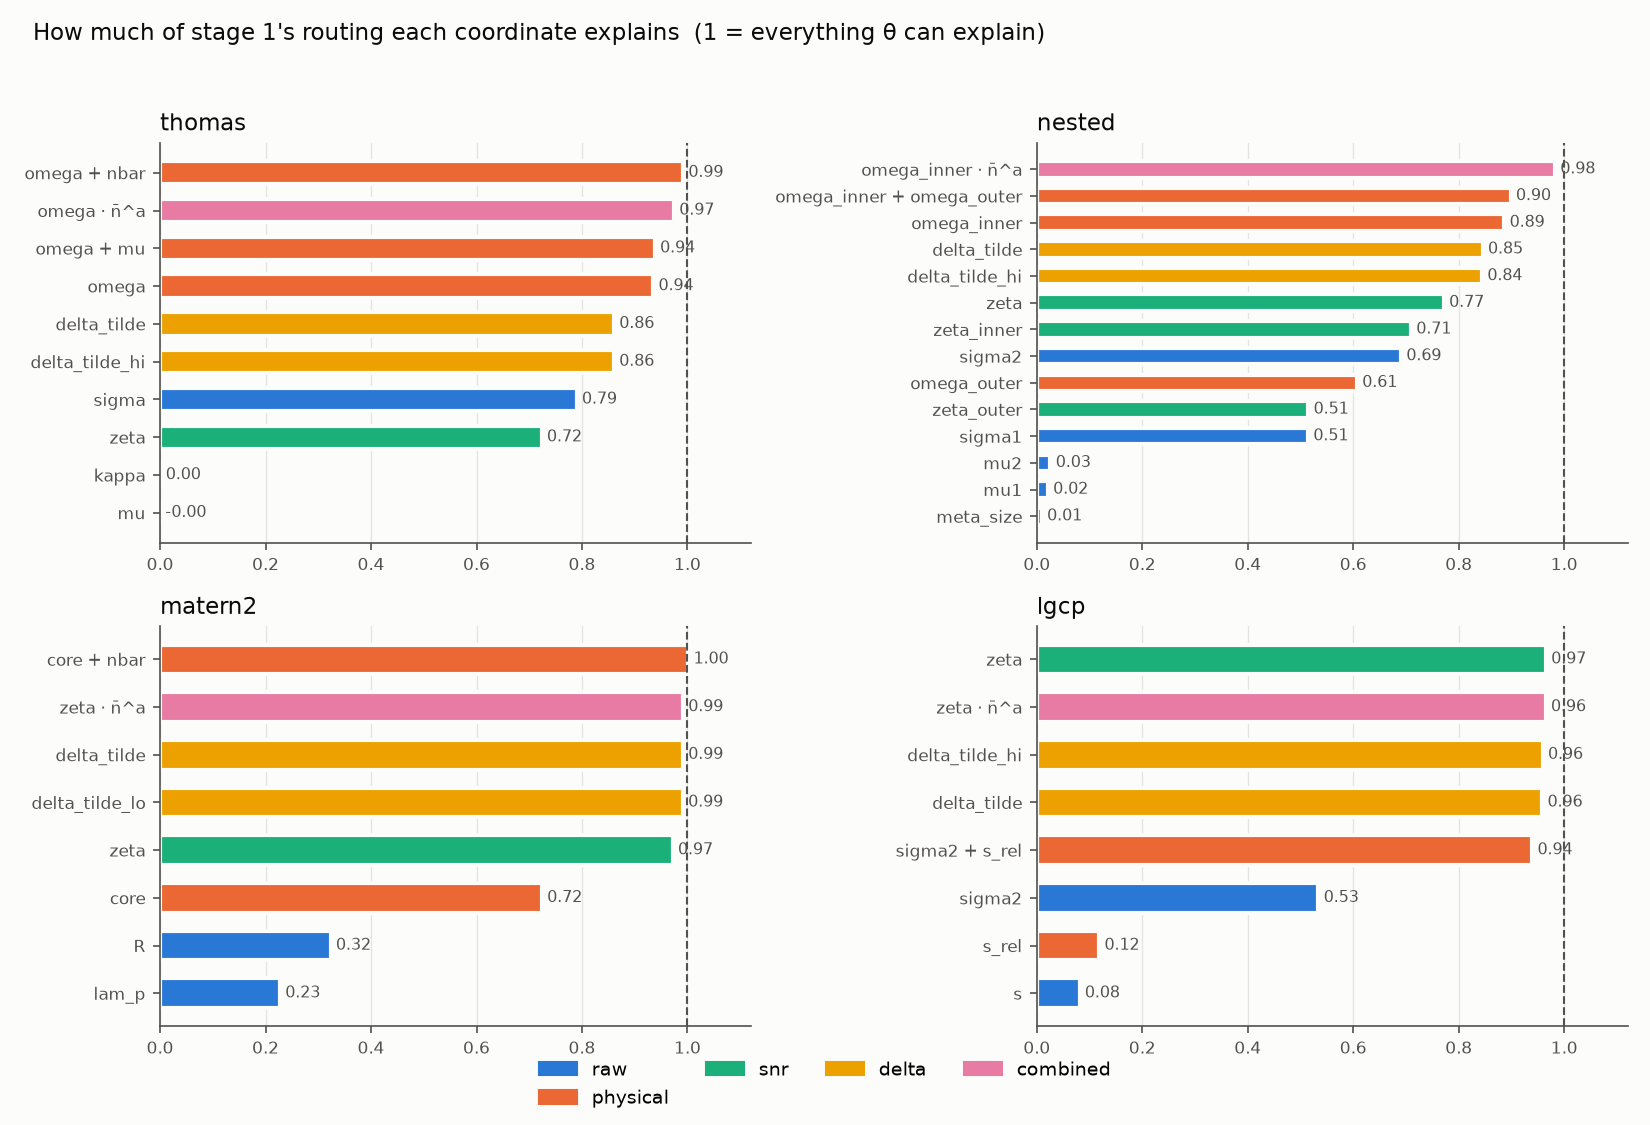
\includegraphics[width=\linewidth]{explained.png}
\end{center}

\subsection*{Result: physical coordinates explain the filter at least as well as $\dt$}
\smallskip
\begin{center}
\begin{tabular}{@{}llrr@{}}
\toprule
family & coordinate & explained & $\dt$ explained \\
\midrule
Thomas    & cluster overlap $\omega=\sigma\sqrt\kappa$, corrected for $\nb$ & 0.975 & 0.861 \\
nested    & inner-cluster overlap, corrected for $\nb$                       & 0.983 & 0.845 \\
Mat\'ern II & hard-core size $\times\,\nb$                                  & 0.992 & 0.991 \\
LGCP      & field strength $\times$ correlation range $\times\,\nb$         & 0.965 & 0.958 \\
\bottomrule
\end{tabular}
\end{center}

\begin{itemize}
  \item \textbf{Interpretable:} whether a Thomas process can be detected depends on how much the clusters \emph{overlap}, not on how many points each has
  \item \textbf{Two-dimensional:} more points make the same overlap easier to see, so each cutoff is on (coordinate, $\nb$), fitted as one combined number coordinate$\,\times\,\nb^{a}$
  \item \textbf{Honest:} $\dt$ is computed from the $L$-function, which the filter also sees, so it has a built-in advantage; physical coordinates that match or beat it are the cleaner choice
\end{itemize}

\begin{center}
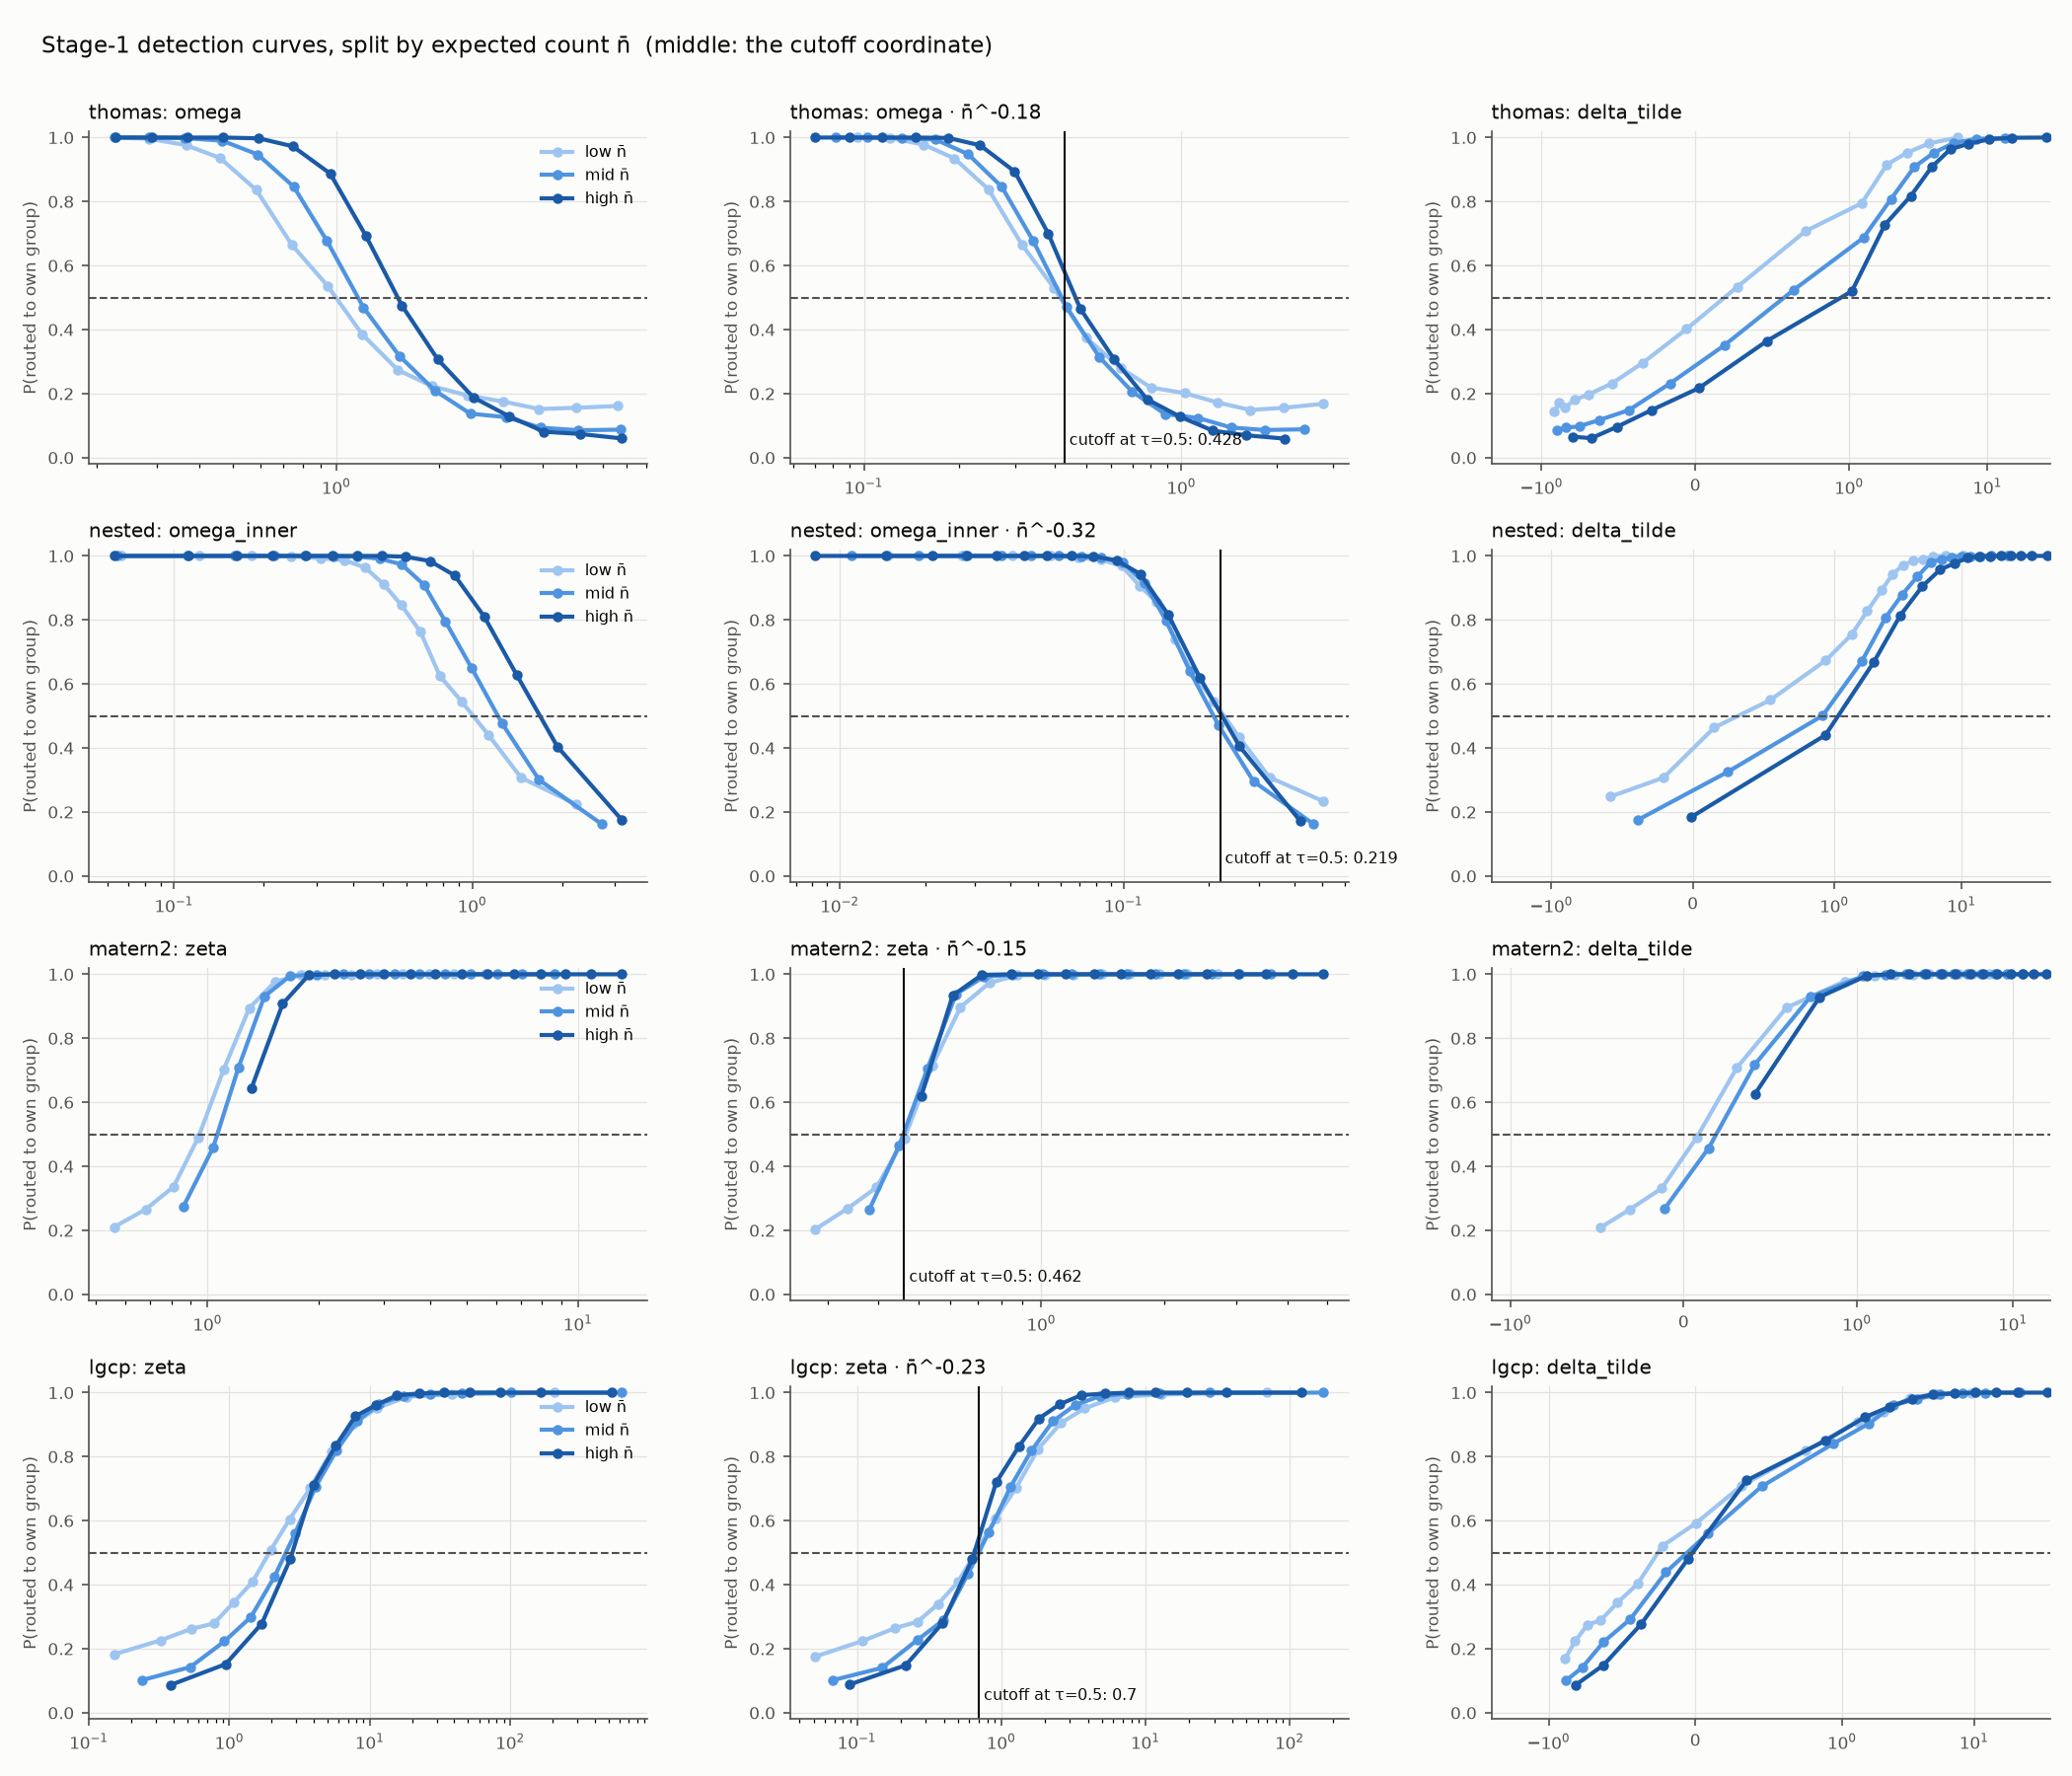
\includegraphics[width=\linewidth]{detection.png}
\end{center}
{\small Left: raw coordinate, curves split by $\nb$. Middle: the $\nb$-corrected coordinate the cutoff uses --- the curves collapse onto one. Right: $\dt$ for comparison.}

\subsection*{The cutoff is a property of the problem, not of the filter}
\begin{center}
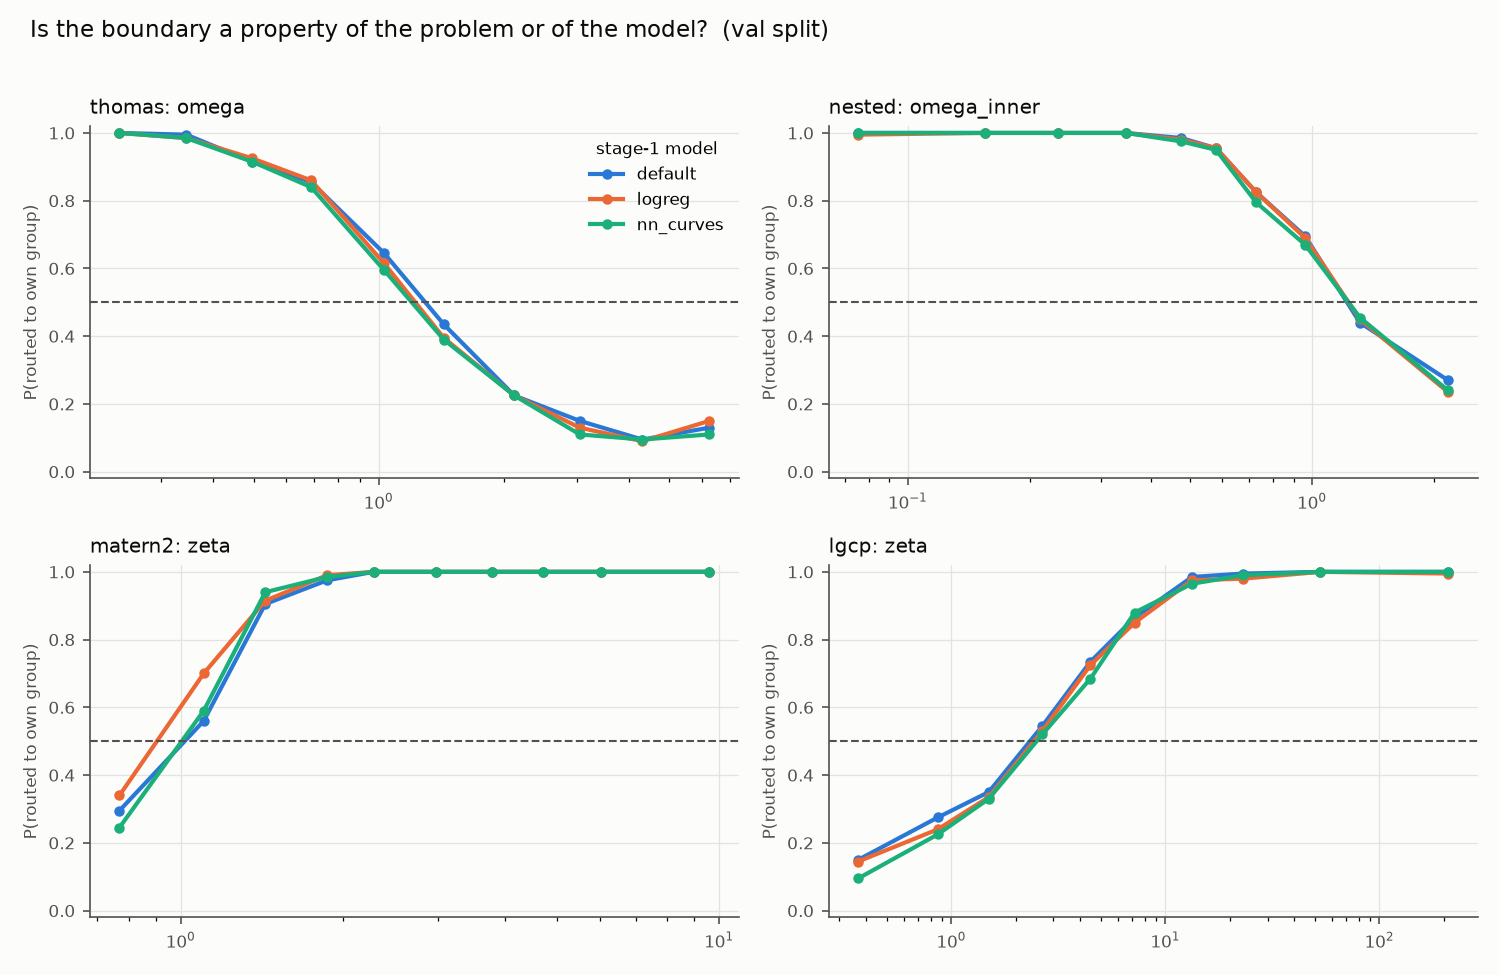
\includegraphics[width=0.85\linewidth]{stability.png}
\end{center}
\begin{itemize}
  \item Trees, logistic regression and the network give the same detection curves
\end{itemize}

\subsection*{From curve to training data}
\begin{itemize}
  \item A pattern is ``past the cutoff'' at threshold $\tau$ if the filter sends patterns like it to their own group with probability $\ge\tau$
  \item $\tau$ is swept over $\{0, 0.3, 0.5, 0.7, 0.9\}$; $\tau=0$ is no filtering, the baseline the filter must beat
  \item Higher $\tau$ = cleaner but fewer training patterns (at $\tau=0.5$: Thomas keeps $49\%$, nested $83\%$, Mat\'ern II $88\%$, LGCP $66\%$)
\end{itemize}

%==============================================================================
\section{Status and open questions}

\begin{itemize}
  \item \textbf{Running:} every stage-2 and stage-3 model at every $\tau$, with trees (done) and the network (in progress), then the assembled pipeline
  \item \textbf{Early result:} a low cutoff ($\tau=0.3$) helps the clustered classifier most; stricter cutoffs lose too much data
  \item \textbf{Thomas vs nested:} their main confusion is identifiability, not features --- a nested process whose outer level is smeared out \emph{is} a Thomas process. Candidate fix: call a pattern nested only when its outer level is visible (the same filter idea, one level down)
  \item \textbf{Impostors:} about $5\%$ of patterns reaching the clustered classifier are not clustered (mostly Poisson). There is no reject option yet; whether that matters is for the end-to-end score to decide
  \item \textbf{End-to-end score:} the first Wasserstein version could not separate the true model from CSR; it is being reworked before it is used to rank pipelines
\end{itemize}

\end{document}
